\documentclass[
  parskip=half,
  bibliography=totoc,     % Literatur im Inhaltsverzeichnis
  captions=tableheading,  % Tabellenüberschriften
  titlepage=firstiscover, % Titelseite ist Deckblatt
]{scrartcl}

% LaTeX2e korrigieren.
\usepackage{fixltx2e}
% Warnung, falls nochmal kompiliert werden muss
\usepackage[aux]{rerunfilecheck}

% deutsche Spracheinstellungen
\usepackage{polyglossia}
\setmainlanguage{german}

% unverzichtbare Mathe-Befehle
\usepackage{amsmath}
% viele Mathe-Symbole
\usepackage{amssymb}
% Erweiterungen für amsmath
\usepackage{mathtools}

% Fonteinstellungen
\usepackage{fontspec}
\defaultfontfeatures{Ligatures=TeX}

\usepackage[
  math-style=ISO,    % \
  bold-style=ISO,    % |
  sans-style=italic, % | ISO-Standard folgen
  nabla=upright,     % |
  partial=upright,   % /
]{unicode-math}

\setmathfont{Latin Modern Math}
\setmathfont[range={\mathscr, \mathbfscr}]{XITS Math}
\setmathfont[range=\coloneq]{XITS Math}
\setmathfont[range=\propto]{XITS Math}
% make bar horizontal, use \hslash for slashed h
\let\hbar\relax
\DeclareMathSymbol{\hbar}{\mathord}{AMSb}{"7E}
\DeclareMathSymbol{ℏ}{\mathord}{AMSb}{"7E}

% richtige Anführungszeichen
\usepackage[autostyle=true,german=quotes]{csquotes}

% Zahlen und Einheiten
\usepackage[
  locale=DE,                   % deutsche Einstellungen
  separate-uncertainty=true,   % Immer Fehler mit \pm
  per-mode=symbol-or-fraction, % m/s im Text, sonst Brüche
  range-phrase=--,
  range-units=single
]{siunitx}


% chemische Formeln
\usepackage[version=3]{mhchem}

% schöne Brüche im Text
\usepackage{xfrac}

% Floats innerhalb einer Section halten
\usepackage[section, below]{placeins}
% Captions schöner machen.
\usepackage[
  labelfont=bf,        % Tabelle x: Abbildung y: ist jetzt fett
  font=small,          % Schrift etwas kleiner als Dokument
  width=0.9\textwidth, % maximale Breite einer Caption schmaler
]{caption}
% subfigure, subtable, subref
\usepackage{subcaption}

% Grafiken können eingebunden werden
\usepackage{graphicx}
% größere Variation von Dateinamen möglich
\usepackage{grffile}

% Standardplatzierung für Floats einstellen
\usepackage{float}
\floatplacement{figure}{htbp}
\floatplacement{table}{htbp}

\usepackage{longtable}

% schöne Tabellen
\usepackage{booktabs}

% Seite drehen für breite Tabellen
\usepackage{pdflscape}

% Literaturverzeichnis
\usepackage[style=numeric,sorting=none,backend=biber]{biblatex}
% Quellendatenbank
\addbibresource{lit.bib}

% Hyperlinks im Dokument
\usepackage[
  unicode,
  pdfusetitle,    % Titel, Autoren und Datum als PDF-Attribute
  pdfcreator={},  % PDF-Attribute säubern
  pdfproducer={}, % "
]{hyperref}
% erweiterte Bookmarks im PDF
\usepackage{bookmark}

% Trennung von Wörtern mit Strichen
\usepackage[shortcuts]{extdash}

\newcommand{\upD}{\mathup{\Delta}}
\newcommand{\upd}{\mathup{d}}

\title{V408: Geometrische Optik}
\author{
  Simon Schulte
  \texorpdfstring{
    \\
    \href{mailto:simon.schulte@udo.edu}{simon.schulte@udo.edu}
  }{}
  \texorpdfstring{\and}{, }
  Tim Sedlaczek
  \texorpdfstring{
    \\
    \href{mailto:tim.sedlaczek@udo.edu}{tim.sedlaczek@udo.edu}
  }{}
}
\publishers{TU Dortmund – Fakultät Physik}

\date{Durchführung: 02.05.2017\\
      Abgabe: 09.05.2017}


\begin{document}

\maketitle
\thispagestyle{empty}
\tableofcontents
\newpage
\setcounter{page}{1}
\section{Zielsetzung}
\label{sec:zielsetzung}
In diesem Versuch sollen die Brennweiten von Linsen und Linsensystemen bestimmt
werden.
\section{Theorie}
\label{sec:theorie}
Die Meisten Linsen bestehen aus Glas. In diesem Versuch wird auch eine mit Wasser
gefüllte Linse verwendet. Entscheidend ist, dass diese Linsen aus einem Material
sind, welches optisch dichter ist als die Umgebung. So wird das Licht an ihren
Oberflächen gebrochen. Dabei ist zwischen zwei Arten von Linsen zu unterscheiden.
Den Sammellinsen, welche wegen ihrer Form das Licht bündeln und eine positive
Brennweite besitzen, und den Streuungslinsen, welche Gegenteiliges bewirken und
eine negative Brennweite besitzen. Bei Sammellinsen entsteht dabei ein reelles
Bild, während bei Streuungslinsen ein virtuelles Bild entsteht (d.h., dass die
Bildweite negativ ist).

\noindent
Wie in Abbildung \ref{fig:V4081} zu sehen ist werden zur Bildkonstruktion
drei Strahlen verwendet, welche sich dadurch auszeichnen, dass sie durch einen
der Brennpunkte oder durch den Mittelpunkt der Linse verlaufen.
Mithilfe der Strahlensätze ergibt sich das so genannte Abbildungsgesetz
\begin{equation}
  V = \frac{B}{G} = \frac{b}{g}.
  \label{eqn:abbildung}
\end{equation}\\
Dabei wird $V$ als Abbildungsmaßstab bezeichnet. $B$ ist die Bildgröße, $G$ die
Gegenstandsgröße, $b$ die Bildweite und $g$ die Gegenstandsweite.
Zusätzlich ergibt sich daraus die Linsengleichung
\begin{equation}
  \frac{1}{f} = \frac{1}{g} + \frac{1}{b}.
  \label{eqn:linsen}
\end{equation}\\
Für dünne Linsen wird vereinfachend angenommen, dass das Licht an der Mittelebene
gebrochen wird. Für dickere Linsen und Linsensysteme gilt dies nicht mehr.
Als Vereinfachung ergeben sich dann zwei Hauptebenen $H$ und $H'$,
für die Bild- und für die Gegenstandsweite, für die die Linsengleichung dann
erfüllt ist.

\noindent
Bei Linsen und Linsensystemen entstehen im Allgemeinen zwei Abbildungsfehler.
Aufgrund der sphärischen Form besitzen Linsen für achsenferne Strahlen
unterschiedliche Brennpunkte, die von der eigentlichen Brennweite abweichen.
Dem kann durch einen speziellen Schliff oder durch eine Irisblende entgegengewirkt
werden.

\noindent
Zudem zeigt sich für verschiedene Wellenlängen im Licht ein unterschiedliches
Brechungsverhalten, weshalb die Brennweite der Linse für verschiedene Farben
variiert.
\clearpage
\section{Durchführung}
\subsection{Versuchsaufbau}
Der Versuchsaufbau besteht aus einer Halogenlampe, einem Gegenstand $G$ (eine
Blende aus L-förmig angeordnetten Kreisblenden), verschiedenen Linsen, zwei
Farbfiltern und einem Schirm, auf den das Bild $B$ projiziert wird.

\noindent
In den Abbildungen \ref{fig:V4081} bis \ref{fig:V4083} sind die schematischen
Aufbauten bzw. die Bildkonstruktionen für die verschiedenen Messungen dargestellt.
\begin{figure}[htb]
  \centering
  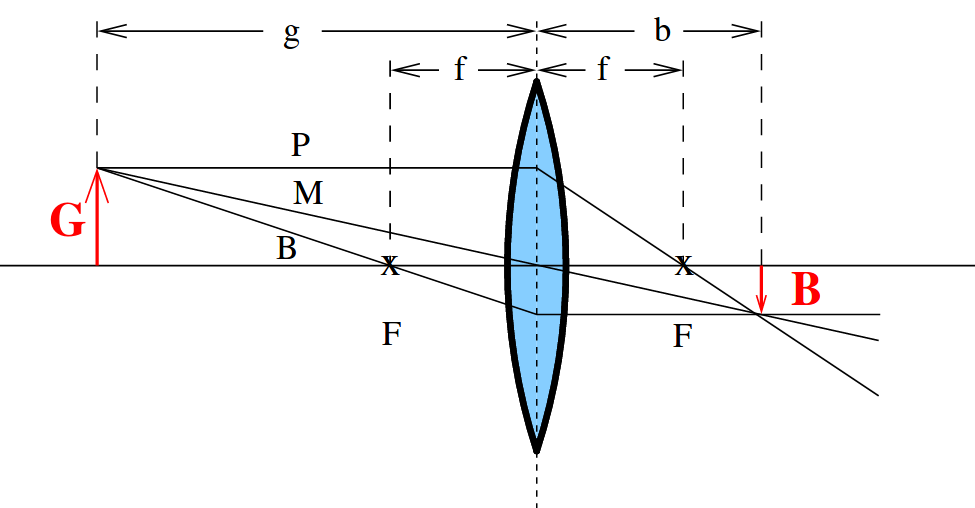
\includegraphics[width=0.8\textwidth]{V4081.png}
  \caption{Aufbau für den ersten Versuchsteil \cite{anleitung}.}
  \label{fig:V4081}
\end{figure}
\begin{figure}[htb]
  \centering
  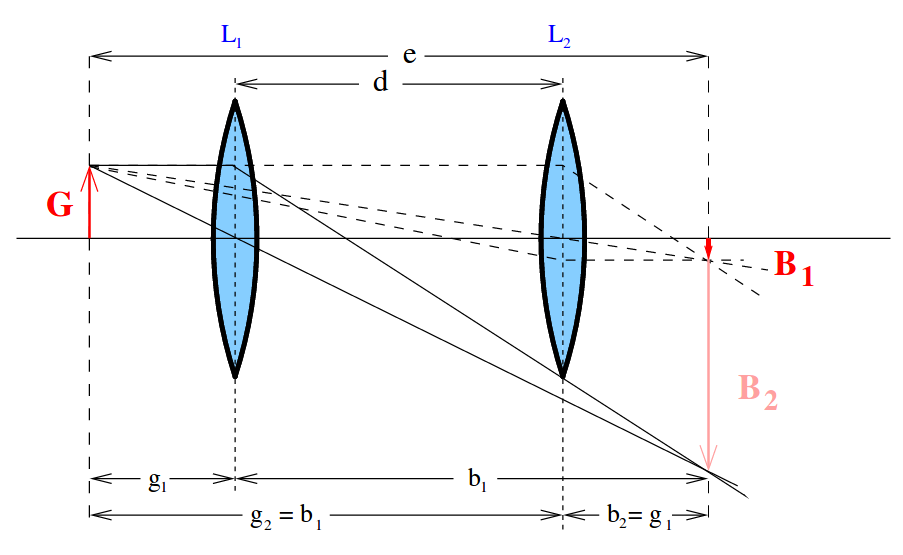
\includegraphics[width=0.8\textwidth]{V4082.png}
  \caption{Aufbau für die Methode von Bessel \cite{anleitung}.}
  \label{fig:V4082}
\end{figure}
\clearpage
\begin{figure}[htb]
  \centering
  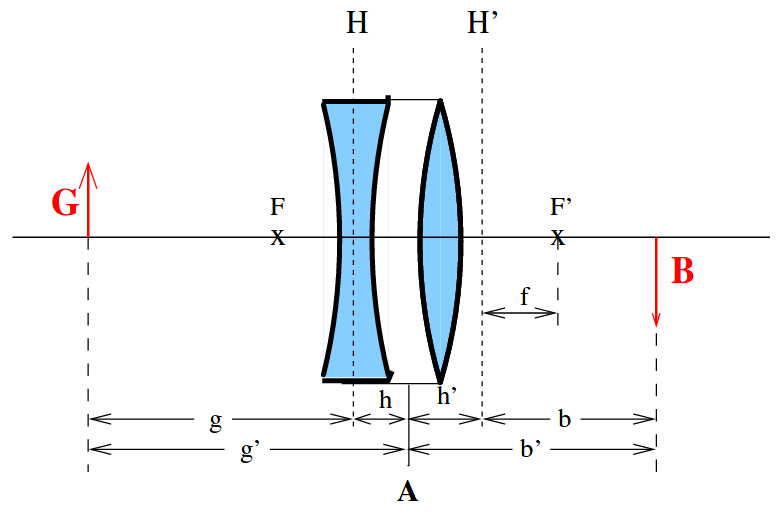
\includegraphics[width=0.8\textwidth]{V4083.png}
  \caption{Aufbau für die Methode von Abbe \cite{anleitung}.}
  \label{fig:V4083}
\end{figure}
\subsection{Versuchsablauf}
Der Versuch besteht aus drei Abschnitten.

\noindent
Zuerst sollen das Abbildungsgesetz und die Linsengleichung überprüft werden.
Hierzu wird eine Linse mit bekannter Brennweite (in unserem Fall \SI{100}{\milli\meter})
verwendet. Diese wird dann in zehn verschiedenen Abständen zum Gegenstand
platziert und entsprechend der Abstand des Schirms für eine scharfe Abbildung
angepasst. Dabei werden die Gegenstandsweite, die Bildweite und bei fünf
Messungen zusätzlich die Bildgröße notiert.
Danach wird die Messung für eine unbekannte Linse wiederholt. Jedoch ohne
dabei die Bildgröße zu notieren.

\noindent
Im zweiten Abschnitt soll die Brennweite einer Linse mit der Methode von
Bessel bestimmt werden. Hierzu wird der Schirm in einem festen Abstand
zum Gegenstand platziert. Aufgrund des festen Abstands gibt es dann zwei
Symmetriepunkte, in denen Bild- und Gegenstandsweite, bei scharfer
Abbildung, die jeweils zum anderen Symmetriepunkt vertauschten Werte
annehmen (wie in Abbildung \ref{fig:V4082} zu sehen). Die Gegenstands-
und Bildweite beider Punkte werden dann für zehn verschiedene Abstände
zwischen Gegenstand und Schirm bestimmt. Anschließend wird die gleiche
Messung jeweils fünf mal mit einem roten und einem blauen Filter vor
dem Gegenstand durchgeführt.

\noindent
Im letzten Abschnitt soll die Brennweite eines Linsensystems mit der Methode
von Abbe bestimmt werden. Hierzu werden zwei Linsen verwendet. Eine Linse
mit einer Brennweite von \SI{-100}{\milli\meter} und eine Linse mit einer
Brennweite von \SI{100}{\milli\meter}. Diese werden möglichst dicht beisammen,
in der Reihenfolge wie sie in Abbildung \ref{fig:V4083} zu sehen ist, zwischen
Gegenstand und Schirm platziert. Nun wird ein Referenzpunkt $A$ gewählt,
von welchem aus im Folgenden immer der Abstand zu Schirm und Gegenstand
bestimmt wird. Die Linsen werden nun in zehn verschiedene Positionen gebracht
und der Schirm für eine scharfe Abbildung verschoben.
Für jede Position der Linsen wird dann der Abstand zum Schirm, der Abstand zum
Gegenstand und der Abbildungsmaßstab (Bildgröße messen und nach \eqref{eqn:abbildung}
ausrechnen) bestimmt.
\section{Auswertung}
\label{sec:auswertung}
Die in der Auswertung verwendeten Mittelwerte mehrfach gemessener Größen sind gemäß der
Gleichung
%
\begin{equation}
    \bar{x}=\frac{1}{n}\sum_{i=1}^n x_i
    \label{eq:mittelwert}
\end{equation}

bestimmt. Die Standardabweichung des Mittelwertes ergibt sich dabei zu

\begin{equation}
    \mathup{\Delta}\bar{x}=\sqrt{\frac{1}{n(n-1)}\sum_{i=1}^n\left(x_i-\bar{x}\right)^2}.
    \label{eq:standardabweichung}
\end{equation}

Resultiert eine Größe über eine Gleichung aus zwei oder mehr anderen fehlerbehafteten Größen, so
berechnet sich der Gesamtfehler nach der Gaußschen Fehlerfortpflanzung zu

\begin{equation}
    \mathup{\Delta}f(x_1,x_2,...,x_n)=\sqrt{\left(\frac{\partial f}{\partial x_1}\mathup{\Delta}x_1\right)^2+\left(\frac{\partial f}{\partial x_2}\mathup{\Delta}x_2\right)^2+ \dotsb +\left(\frac{\partial f}{\partial x_n}\mathup{\Delta}x_n\right)^2}.
    \label{eq:fehlerfortpflanzung}
\end{equation}

Alle in der Auswertung angegebenen Größen sind stets auf die erste signifikante Stelle des
Fehlers gerundet. Setzt sich eine Größe über mehrere Schritte aus anderen Größen zusammen,
so wird erst am Ende gerundet, um Fehler zu vermeiden. Zur Auswertung wird das Programm Python verwendet.
\subsection{Bestimmung der Brennweite von einer Linse durch Messung der Gegenstandsweite und der Bildweite}

Zunächst wird die Brennweite von einer Sammellinse durch Messung der Gegenstands- und Bildweite unter
Zuhilfenahme der in Abschnitt~\ref{sec:theorie} beschriebenen Linsengleichung~\eqref{eqn:linsen}
bestimmt. Tabelle~\ref{tab:a} beinhaltet die dazu aufgenommenen Werte~$(g,b)$, sowie
die berechneten Brennweiten~$f$. Als Mittelwert ergibt sich daraus für die Linse bekannter Brennweite

\begin{equation}
f_{\text{Linse 1}} = \SI{75.3(2)}{\milli\metre}
\end{equation}

\begin{table}[htp]
	\begin{center}
	\caption{Messwerte zur Bestimmung der Gegenstandsweiten der Wasserlinse mit unbekannter Brennweite.}
	\label{tab:b}
		\begin{tabular}{cccccc}
			\toprule
			{$g[\si{\milli\metre}]$} & {$b[\si{\milli\metre}]$} & {$f[\si{\milli\metre}]$}\\
			\midrule
			$330$ & $98$ & $75.56$ \\
			$320$ & $99$ & $75.60$ \\
			$310$ & $100$ & $75.61$ \\
			$300$ & $100$ & $75.00$ \\
			$290$ & $101$ & $74.91$ \\
			$280$ & $102$ & $74.76$\\
			$270$ & $105$ & $75.60$\\
			$260$ & $106$ & $75.30$\\
			$250$ & $107$ & $74.93$\\
			$240$ & $110$ & $75.43$\\
			\bottomrule
		\end{tabular}
	\end{center}
\end{table}
Nun wird das gleiche für eine Linse mit unbekannter Brennweite durchgeführt.
Tabelle~\ref{tab:b} beinhaltet die dazu aufgenommenen Werte~$(g,b)$, sowie
die berechneten Brennweiten~$f$. Als Mittelwert ergibt sich daraus für die Linse bekannter Brennweite
\begin{equation}
f_{\text{Linse 2}} = \SI{96.5(3)}{\milli\metre}
\end{equation}

\begin{table}[htp]
	\begin{center}
	\caption{Messwerte zur Bestimmung der Gegenstandsweiten der Linse mit bekannter Brennweite.}
	\label{tab:a}
		\begin{tabular}{cccccc}
			\toprule
			{$g[\si{\milli\metre}]$} & {$b[\si{\milli\metre}]$} &
      {$f[\si{\milli\metre}]$}\\
			\midrule
			$330$ & $136$ & $96.31$\\
			$320$ & $139$ & $96.91$\\
			$310$ & $140$ & $96.44$\\
			$300$ & $143$ & $96.84$\\
			$290$ & $144$ & $96.22$\\
			$280$ & $146$ & $95.96$\\
			$270$ & $150$ & $96.43$\\
			$260$ & $154$ & $96.71$\\
			$250$ & $157$ & $96.44$\\
			$240$ & $161$ & $96.36$\\
			\bottomrule
		\end{tabular}
	\end{center}
\end{table}

Die angegebenen Fehler sind hierbei die statistischen Fehler der Mittelwerte. Um neben dem statistischen
Fehler ein weiteres Maß für die Messgenauigkeit zu erhalten, werden die gemessenen Gegenstandsweiten auf
der x-Achse eines Koordinatensystems notiert und mit ihren entsprechenden Bildweiten, die auf der y-Achse
notiert sind, verbunden. Der Schnittpunkt der Geraden markiert die Brennweite der Linse. Je genauer sich
die Geraden in einem Punkt treffen, desto präziser wurde gemessen. Abbildung~\ref{fig:plot_1}
zeigt dieses Koordinatensystem für die Bestimmung der Brennweite der bekannten Linse, Abbildung
\ref{fig:plot_2} zeigt dies für die Wasserlinse unbekannter Brennweite.

\begin{figure}[H]
    \centering
    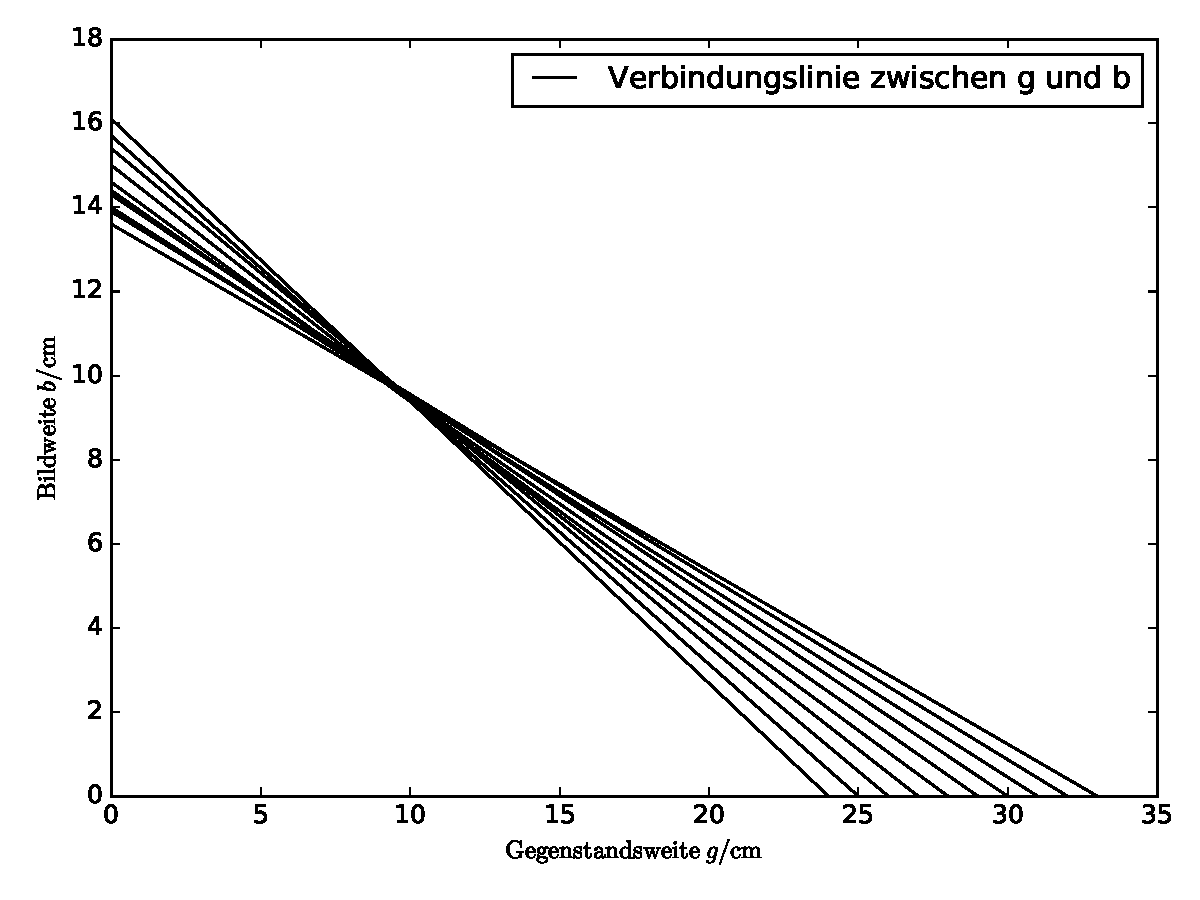
\includegraphics[width=0.85\textwidth]{sam.pdf}
    \caption{Graphische Veranschaulichung der Messgenauigkeit für die Untersuchung der Linse mit bekannter Brennweite.}
    \label{fig:plot_1}
\end{figure}

\begin{figure}[H]
    \centering
    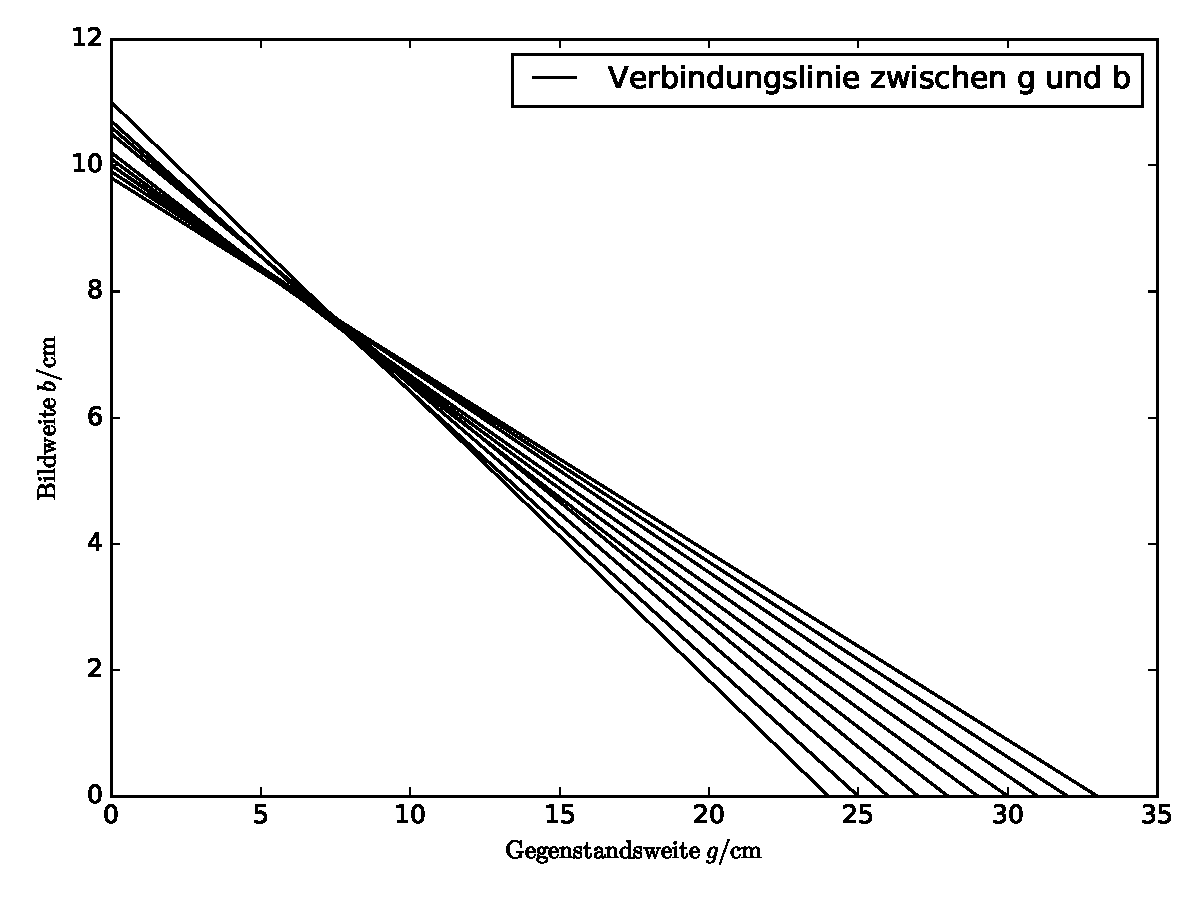
\includegraphics[width=0.85\textwidth]{sam1.pdf}
    \caption{Graphische Veranschaulichung der Messgenauigkeit für die Untersuchung der Wasserlinse mit unbekannter Brennweite.}
    \label{fig:plot_2}
\end{figure}

\subsection{Bestimmung der Brennweite einer Linse nach der Methode von Bessel}

Für die Bestimmung der Brennweite einer Linse mit der Methode von Bessel werden bei festem
Abstand zwischen Gegenstand und Bild zwei Positionen für die zu untersuchende Linse im Strahlengang
gesucht, bei denen das Bild eine maximale Schärfe erreicht. Abbildung~\ref{fig:V4082} veranschaulicht
die geometrische Beziehungen der im Folgenden benutzten Größen. Dabei bezeichnet $e$ den gemessenen
Gesamtabstand zwischen Gegenstand und Bild, $g_1$ und $b_1$ Gegenstands- bzw. Bildweite, wenn die Linse
näher am Gegenstand als am Bild positioniert ist und $g_2$ und $b_2$ Gegenstands- bzw. Bildweite, wenn
sich die Linse näher am Bild befindet.

Aufgrund der Symmetrien $e=g_1+b_1=g_2+b_2$ und $d=g_1-b_1=g_2-b_2$ folgt durch Umformen der
Linsengleichung für die Brennweite $f$ die Beziehung

\begin{equation}
    f=\frac{e^2-d^2}{4e}.
\end{equation}

Die Untersuchung ergibt bei der Verwendung von weißem Licht die in
Tabelle~\ref{tab:weiss} aufgeführten Werte. Es ergeben sich somit stets zwei Brennweiten
pro eingestelltem Gesamtabstand $e$. Wie im Abschnitt zuvor folgt aus den errechneten Brennweiten die
Brennweite der Linse im Mittel, sowie der Fehler des Mittelwerts. Es ist

\begin{equation}
    f_{\text{weiß}} = \SI{96.41(9)}{\milli\metre}.
\end{equation}
In einem weiteren Schritt wird die Brennweite der Linse für rotes und blaues Licht bestimmt. Die
Vorgehensweise ist analog zur Untersuchung mit weißem Licht. Die Tabellen~\ref{tab:rot}
und~\ref{tab:blau} zeigen die aufgenommenen Messdaten für rotes und blaues Licht. Es
ergibt sich für die Brennweiten
%
\begin{align}
    f_{\text{rot}} = \SI{96.6(3)}{\milli\metre}\\
    &f_{\text{rot}} = \SI{96.4(3)}{\milli\metre}.
\end{align}

\begin{table}[htp]
	\begin{center}
	\caption{Messwerte zur Bestimmung der Brennweite einer Linsen mit der Methode von Bessel. Es wurde weisses Licht verwendet.}
	\label{tab:weiss}
		\begin{tabular}{ccccccc}
			\toprule
			\multicolumn{7}{c}{Linse 1, $f=\SI{100}{\milli\metre}$, weisses Licht}\\
			{$e[\si{\milli\metre}]$} & {$g_1[\si{\milli\metre}]$} & {$b_1[\si{\milli\metre}]$} & {$g_2[\si{\milli\metre}]$} & {$b_2[\si{\milli\metre}]$} & \multicolumn{2}{c}{$f[\si{\milli\metre}]$}\\
			\midrule
			$390$ & $220$ & $170$ & $170$ & $220$ & $95.90$ & $95.90$\\
			$400$ & $240$ & $160$ & $163$ & $237$ & $96.00$ & $96.58$\\
			$410$ & $253$ & $157$ & $154$ & $256$ & $96.88$ & $96.16$\\
			$420$ & $270$ & $150$ & $152$ & $268$ & $96.42$ & $96.99$\\
			$430$ & $285$ & $145$ & $146$ & $284$ & $96.10$ & $96.43$\\
			$440$ & $298$ & $142$ & $143$ & $297$ & $96.17$ & $96.53$\\
			$450$ & $310$ & $140$ & $140$ & $310$ & $96.44$ & $96.44$\\
			$460$ & $322$ & $138$ & $139$ & $321$ & $96.60$ & $97.00$\\
			$470$ & $335$ & $135$ & $136$ & $334$ & $96.22$ & $96.65$\\
			$480$ & $347$ & $133$ & $134$ & $346$ & $96.15$ & $96.59$\\
			\bottomrule
		\end{tabular}
	\end{center}
\end{table}

\begin{table}[htp]
	\begin{center}
	\caption{Messwerte zur Bestimmung der Brennweite einer Linsen mit der Methode von Bessel. Es wurde rotes Licht verwendet.}
	\label{tab:rot}
		\begin{tabular}{ccccccc}
			\toprule
			\multicolumn{7}{c}{Linse 1, $f=\SI{100}{\milli\metre}$, rotes Licht}\\
			{$e[\si{\milli\metre}]$} & {$g_1[\si{\milli\metre}]$} & {$b_1[\si{\milli\metre}]$} & {$g_2[\si{\milli\metre}]$} & {$b_2[\si{\milli\metre}]$} & \multicolumn{2}{c}{$f[\si{\milli\metre}]$}\\
			\midrule
      $440$ & $299$ & $141$ & $142$ & $298$ & $95.82$ & $96.17$\\
      $450$ & $310$ & $140$ & $140$ & $310$ & $96.44$ & $96.44$\\
      $460$ & $322$ & $138$ & $138$ & $322$ & $96.60$ & $96.60$\\
      $470$ & $333$ & $137$ & $136$ & $334$ & $97.07$ & $96.65$\\
      $480$ & $345$ & $135$ & $135$ & $345$ & $97.03$ & $97.03$\\
      \bottomrule
		\end{tabular}
	\end{center}
\end{table}

\begin{table}[htp]
	\begin{center}
	\caption{Messwerte zur Bestimmung der Brennweite einer Linsen mit der Methode von Bessel. Es wurde blaues Licht verwendet.}
	\label{tab:blau}
		\begin{tabular}{ccccccc}
			\toprule
			\multicolumn{7}{c}{Linse 1, $f=\SI{100}{\milli\metre}$, blaues Licht}\\
			{$e[\si{\milli\metre}]$} & {$g_1[\si{\milli\metre}]$} & {$b_1[\si{\milli\metre}]$} & {$g_2[\si{\milli\metre}]$} & {$b_2[\si{\milli\metre}]$} & \multicolumn{2}{c}{$f[\si{\milli\metre}]$}\\
			\midrule
			$440$ & $298$ & $142$ & $144$ & $296$ & $96.17$ & $96.87$\\
			$450$ & $310$ & $140$ & $141$ & $309$ & $96.44$ & $96.82$\\
			$460$ & $323$ & $137$ & $138$ & $322$ & $96.20$ & $96.60$\\
			$470$ & $334$ & $136$ & $136$ & $334$ & $96.65$ & $96.65$\\
			$480$ & $347$ & $133$ & $132$ & $348$ & $96.15$ & $95.70$\\
			\bottomrule
		\end{tabular}
	\end{center}
\end{table}

\newpage
\subsection{Untersuchung eines Linsensystems nach der Methode von Abbe}

Die Untersuchung der Brennweite eines Linsensystems, bestehend aus einer Zerstreuungslinse mit
$f=\SI{-100}{\milli\metre}$ und einer Sammellinse mit $f=\SI{100}{\milli\metre}$, erfolgt mit der
Methode von Abbe. Da die Lage der Hauptebenen des Linsensystems zunächst unbekannt ist, wird ein
Referenzpunkt $A$ gewählt, hinsichtlich dem Gegenstandsweite $g'$ und Bildweite $b'$ bestimmt werden. Die
im Folgenden verwendeten Größen können der Abbildung~\ref{fig:V4083} entnommen werden. Aus der Anordnung
und durch Umformung der Gleichungen~\eqref{eqn:abbildung} und~\eqref{eqn:linsen} folgen die
Beziehungen

\begin{align}
    g'&=g+h=f\cdot\left(1+\frac{1}{V}\right)+h \\
    b'&=b+h'=f\cdot(1+V)+h'
\end{align}

aus denen sich durch lineare Ausgleichsrechnung die Brennweite $f$ ermitteln lässt. Die zugehörigen
Messdaten sind in Tabelle~\ref{tab:abbe} gelistet. Neben den Gegenstandsweiten $g'$, den
Bildweiten $b'$ sind auch stets die Abbildungsmaßstäbe $V$ angegeben, die sich
gemäß der Beziehung $V=\sfrac{B}{G}$ bei immer gleicher Gegenstandsgröße $G=\SI{30.0}{\milli\metre}$
bestimmen lassen.

\begin{table}[htp]
	\begin{center}
	\caption{Messwerte zur Bestimmung der Brennweite eines Linsensystems mit der Methode von Abbe.}
	\label{tab:abbe}
		\begin{tabular}{ccc}
			\toprule
			 {$V$} & {$g'[\si{\milli\metre}]$} & {$b'[\si{\milli\metre}]$}\\
			\midrule
			$2.2$ & $190$ & $633$\\
			$3.2$ & $166$ & $792$\\
			$1.6$ & $215$ & $526$\\
			$1.4$ & $225$ & $495$\\
			$1.3$ & $235$ & $470$\\
			$1.2$ & $245$ & $449$\\
			$1.1$ & $255$ & $446$\\
			$1.0$ & $265$ & $428$\\
			$1.0$ & $275$ & $416$\\
			$0.9$ & $285$ & $415$\\
			\bottomrule
		\end{tabular}
	\end{center}
\end{table}


Die Ausgleichsrechnung der Messwerte liefert die in Abbildung~\ref{fig:plot_abbe_1}
bzw.~\ref{fig:plot_abbe_2} durch die Messpunkte gelegten Ausgleichsgeraden. Steigung und
y-Achsenabschnitt liefern direkt die in Abbildung~\ref{fig:V4083} unbekannten Größen. Die angegebenen
Fehler resultieren aus den Ungenauigkeiten der Ausgleichsrechnung. Es ist

\begin{align*}
    f  &= \SI{121(3)}{\milli\metre}\\
    f' &= \SI{264(5)}{\milli\metre}\\
    h  &= \SI{14.8(4)}{\milli\metre}\\
    h' &= \SI{16.8(3)}{\milli\metre}.
\end{align*}

Aus der Richtung des Gegenstandes gesehen liegt die erste Hauptebene somit um $h$ vor dem frei gewählten
Referenzpunkt, die zweite Hauptebene um $h'$ dahinter. $f$ bzw. $f'$ ist der Abstand des jeweiligen vor
oder hinter der Hauptebene liegenden Brennpunktes.

\begin{figure}[H]
    \centering
    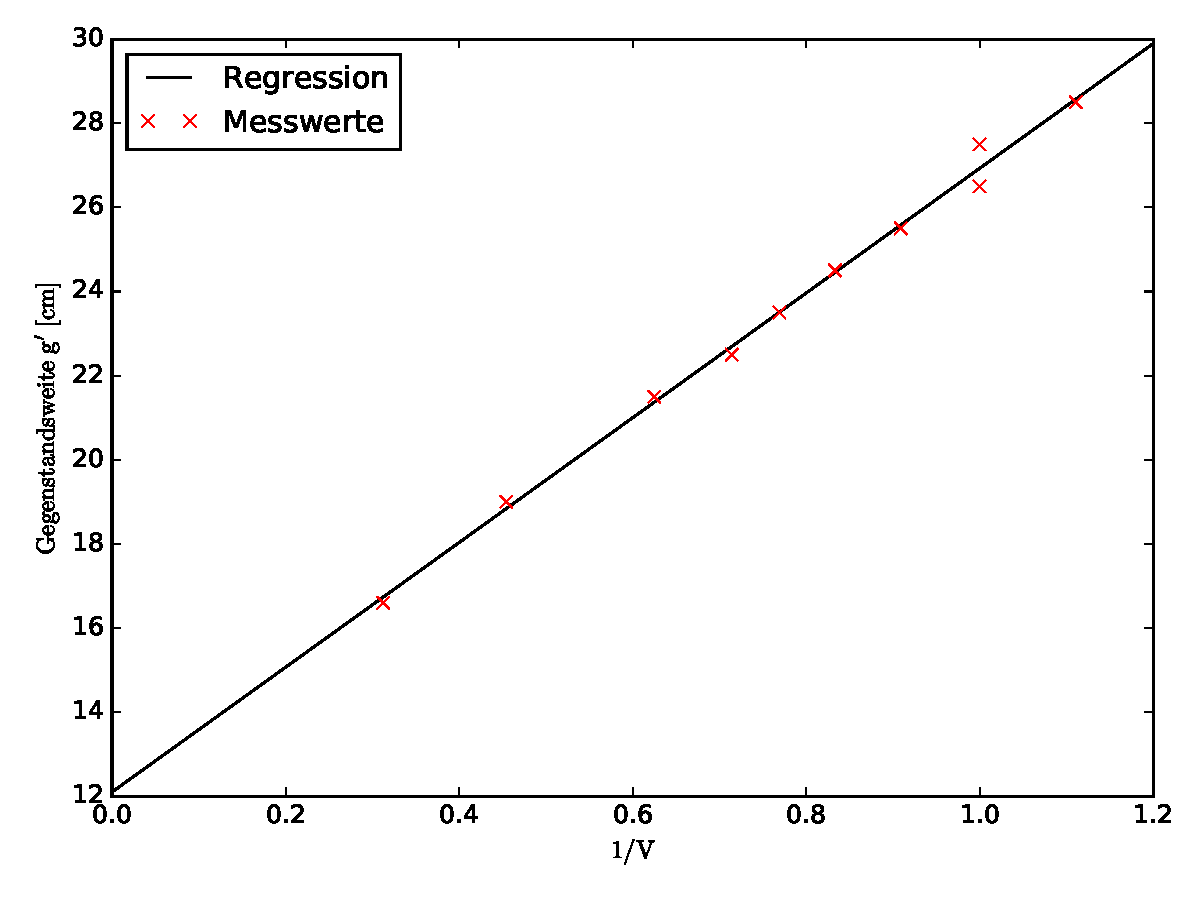
\includegraphics[width=0.8\textwidth]{AbbeV.pdf}
    \caption{Lineare Regression der Messwerte zur Bestimmung von $f$ und $h$ aus den Gegenstandsweiten $g'$ und den Abbildungsverhältnissen $V$.}
    \label{fig:plot_abbe_1}
\end{figure}

\begin{figure}[H]
    \centering
    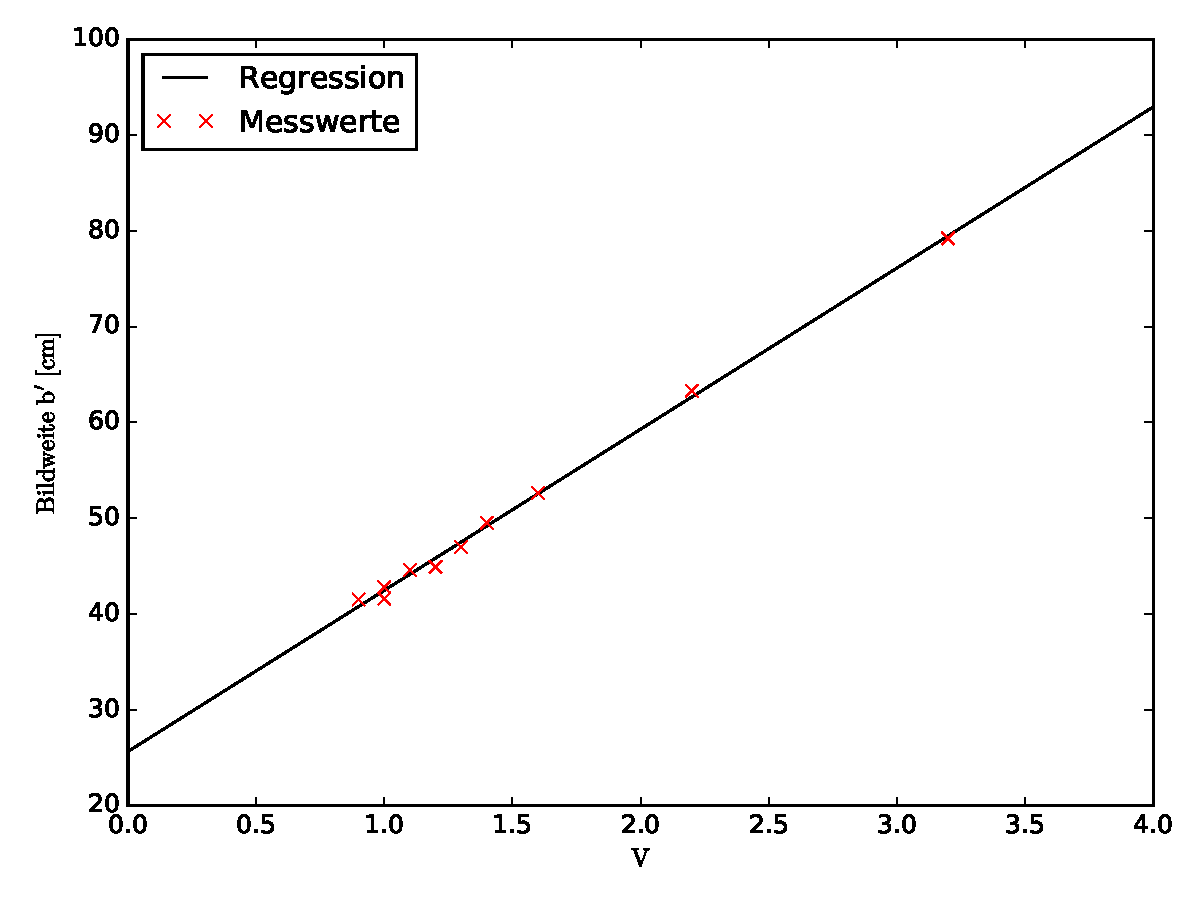
\includegraphics[width=0.8\textwidth]{AbbeV2.pdf}
    \caption{Lineare Regression der Messwerte zur Bestimmung von $f'$ und $h'$ aus den Bildweiten $b'$ und den Abbildungsverhältnissen $V$.}
    \label{fig:plot_abbe_2}
\end{figure}
\section{Diskussion}
\label{sec:diskussion}
Im Folgenden sollen die Ergebnisse aus Abschnitt~\ref{sec:auswertung} soweit möglich anhand der Gerätedaten
diskutiert werden. Sowohl bei der Bestimmung der Brennweite durch einfache Messung der Gegenstands- und
Bildweite, als auch bei der Bestimmung der Brennweite nach Bessel wird eine bekannte Linse mit
Brennweite $f=\SI{100}{\milli\metre}$ verwendet. Die Untersuchung ergibt den gemittelten Wert
$\SI{75.3(2)}{\milli\metre}$. Es ist zu erkennen, dass das
Ergebnis relativ nah an dem angegeben Wert liegt. Der Wert ist kleiner, was entweder auf einen
systematischen Fehler beim Experimentieren, oder auf eine tatsächliche Abweichung der Brennweite im Rahmen
der vom Hersteller angegebenen Toleranz hindeutet. Die bekannte Genauigkeit der Messung für die Linse mit
$f=\SI{100}{\milli\metre}$ ermöglicht auch eine qualitative Aussage über die Messgenauigkeit bei der
Untersuchung der Wasserlinse. Es ist davon auszugehen, dass hier die ermittelte Brennweite von $f_{\text{Wasserlinse}} = \SI{96.5(3)}{\milli\metre}$
 nah am tatsächlichen Wert liegt.

Bei der Untersuchung der chromatischen Aberration im zweiten Versuchsteil ergeben sich nahzu identische
Brennweiten für rotes und blaues Licht. Die Abweichung zum weißen Licht ist ebenfalls minimal. Es scheint,
dass der Effekt zu klein oder die Linse zu gut geschliffen ist, als dass er im Experiment ausschlaggebend beobachtet werden
kann.

Die Untersuchung des Linsensystems nach der Methode von Abbe liefert für die Brennweite im Mittel
den Wert $f=\SI{193}{\milli\metre}$. Insgesamt scheint auch diese Messung im
Rahmen normaler statistischer Schwankungen gute Ergebnisse zu liefern. Es zeigt sich, dass die Brennweite
von Linsen oder Linsensystemen mit verschiedenen Methoden und mit wenig Aufwand genau bestimmt werden können.
\clearpage
\nocite{*}
\printbibliography

\end{document}
